\documentclass{mimosis}

\usepackage{metalogo}

%%%%%%%%%%%%%%%%%%%%%%%%%%%%%%%%%%%%%%%%%%%%%%%%%%%%%%%%%%%%%%%%%%%%%%%%
% Some of my favourite personal adjustments
%%%%%%%%%%%%%%%%%%%%%%%%%%%%%%%%%%%%%%%%%%%%%%%%%%%%%%%%%%%%%%%%%%%%%%%%
%
% These are the adjustments that I consider necessary for typesetting
% a nice thesis. However, they are *not* included in the template, as
% I do not want to force you to use them.

% This ensures that I am able to typeset bold font in table while still aligning the numbers
% correctly.
\usepackage{etoolbox}

%%%%%%%%%%%%%%%%%%%%%%%%%%%%%%%%%%%%%%%%%%%%%%%%%%%%%%%%%%%%%%%%%%%%%%%%
% Hyperlinks & bookmarks
%%%%%%%%%%%%%%%%%%%%%%%%%%%%%%%%%%%%%%%%%%%%%%%%%%%%%%%%%%%%%%%%%%%%%%%%

\usepackage[%
  colorlinks = true,
  citecolor  = RoyalBlue,
  linkcolor  = RoyalBlue,
  urlcolor   = RoyalBlue,
  unicode,
  ]{hyperref}

  \usepackage{bookmark}

  %%%%%%%%%%%%%%%%%%%%%%%%%%%%%%%%%%%%%%%%%%%%%%%%%%%%%%%%%%%%%%%%%%%%%%%%%
  % Bibliography
  %%%%%%%%%%%%%%%%%%%%%%%%%%%%%%%%%%%%%%%%%%%%%%%%%%%%%%%%%%%%%%%%%%%%%%%%
  %
  % I like the bibliography to be extremely plain, showing only a numeric
  % identifier and citing everything in simple brackets. The first names,
  % if present, will be initialized. DOIs and URLs will be preserved.



  %%%%%%%%%%%%%%%%%%%%%%%%%%%%%%%%%%%%%%%%%%%%%%%%%%%%%%%%%%%%%%%%%%%%%%%%
  % Fonts
  %%%%%%%%%%%%%%%%%%%%%%%%%%%%%%%%%%%%%%%%%%%%%%%%%%%%%%%%%%%%%%%%%%%%%%%%

  \ifxetexorluatex
  \usepackage{unicode-math}
  \setmainfont{EB Garamond}
  \setmathfont{Garamond Math}

  % Load some missing symbols from another font.
  \setmathfont{STIX Two Math}[%
    range = {
      \sharp,
      \natural,
      \flat,
      \clubsuit,
      \spadesuit,
      \checkmark
    }
    ]
    \setmonofont[Scale=MatchLowercase]{Source Code Pro}
    \else
    \usepackage[lf]{ebgaramond}
    \usepackage[oldstyle,scale=0.7]{sourcecodepro}
    \singlespacing
    \fi



    %%%%%%%%%%%%%%%%%%%%%%%%%%%%%%%%%%%%%%%%%%%%%%%%%%%%%%%%%%%%%%%%%%%%%%%%
    % Ordinals
    %%%%%%%%%%%%%%%%%%%%%%%%%%%%%%%%%%%%%%%%%%%%%%%%%%%%%%%%%%%%%%%%%%%%%%%%

    \makeatletter
    \@ifundefined{st}{%
      \newcommand{\st}{\textsuperscript{\textup{st}}\xspace}
      }{}
      \@ifundefined{rd}{%
        \newcommand{\rd}{\textsuperscript{\textup{rd}}\xspace}
        }{}
        \@ifundefined{nd}{%
          \newcommand{\nd}{\textsuperscript{\textup{nd}}\xspace}
          }{}
          \makeatother

          \renewcommand{\th}{\textsuperscript{\textup{th}}\xspace}

          %%%%%%%%%%%%%%%%%%%%%%%%%%%%%%%%%%%%%%%%%%%%%%%%%%%%%%%%%%%%%%%%%%%%%%%%
          % Incipit
          %%%%%%%%%%%%%%%%%%%%%%%%%%%%%%%%%%%%%%%%%%%%%%%%%%%%%%%%%%%%%%%%%%%%%%%%

          \title{{CPU-Scheduling}}
          \subtitle{What waiting in line at the supermarket and your computer have in common}
          \author{Mark Krutzler 4a}


          %%%%%%%%%%%%%%%%%%%%%%%%%%%%%%%%%%%%%%%%%%%%%%%%%%%%%%%%%%%%%%%%%%%%%%%%
          % Code Blocks
          %%%%%%%%%%%%%%%%%%%%%%%%%%%%%%%%%%%%%%%%%%%%%%%%%%%%%%%%%%%%%%%%%%%%%%%%

          \usepackage{minted}

          \usepackage{hyperref}

          % SVG support
          \usepackage{svg}

          \begin{document}

          \frontmatter
          \begin{titlepage}
    \vspace*{5cm}
    \makeatletter
    \begin{center}
      \textsc{Kantonsschule Im Lee, Winterthur}\\
      \vspace*{1cm}
      \begin{Huge}
        \@title
      \end{Huge}\\[0.1cm]
      %
      \begin{Large}
        \@subtitle
      \end{Large}\\
      %
      \emph{by}
      \@author\\
      \emph{under the supervision of}
      Thomas Graf\\
      %
      \vfill
      06. January 2025
    \end{center}
    \makeatother
\end{titlepage}
  
\newpage
\null
\thispagestyle{empty}
\newpage
  

          %\begin{center}
  \textsc{Abstract}
\end{center}
%
\noindent
%
Abstract here

          \tableofcontents
          \listoffigures


          \mainmatter


          %%%%%%%%%%%%%%%%%%%%%%%%%%%%%%%%%%%%%%%%%%%%%%%%%%%%%%%%%%%%%%%%%%%%%%%%
\chapter{How do we compare policies}
%%%%%%%%%%%%%%%%%%%%%%%%%%%%%%%%%%%%%%%%%%%%%%%%%%%%%%%%%%%%%%%%%%%%%%%%

%%%%%%%%%%%%%%%%%%%%%%%%%%%%%%%%%%%%%%%%%%%%%%%%%%%%%%%%%%%%%%%%%%%%%%%%
\chapter{Initial Problem}
%%%%%%%%%%%%%%%%%%%%%%%%%%%%%%%%%%%%%%%%%%%%%%%%%%%%%%%%%%%%%%%%%%%%%%%%

%%%%%%%%%%%%%%%%%%%%%%%%%%%%%%%%%%%%%%%%%%%%%%%%%%%%%%%%%%%%%%%%%%%%%%%%
\chapter{Evolving Supermarket}
%%%%%%%%%%%%%%%%%%%%%%%%%%%%%%%%%%%%%%%%%%%%%%%%%%%%%%%%%%%%%%%%%%%%%%%%

%%%%%%%%%%%%%%%%%%%%%%%%%%%%%%%%%%%%%%%%%%%%%%%%%%%%%%%%%%%%%%%%%%%%%%%%
\chapter{Example}
%%%%%%%%%%%%%%%%%%%%%%%%%%%%%%%%%%%%%%%%%%%%%%%%%%%%%%%%%%%%%%%%%%%%%%%%

          \chapter{Predicting the Future}

\section{Idea}

The first policy we look at is formerly called Multi-Level Feedback Queue or MLFQ short. The create Fernando J. Corbató recieved a Turning Award for it in 1990. 
As the title already says, this policy tries to predict the future behaviour of the processes based on the past.
A job can be generally act in two ways.
Either it is a resources intensive crunching problem (think about exporting a video or compiling code) or it is a program, which needs quick response time (think about your text editor).
In reality most jobs jump between these two states.
We usually want to give the response based processes priority, because that is what the user interacts with and it is here that he primarily feels a delay.

The policy is based on multiple queues, which have each different priorities.
Each process gets assigned to a queue. There are however not set in stone
Based on the reasons above we want to assume that a new process is responsive, because in the worst case scenario, we need to just demote the non-responsive ones.
If however a process turns out to be interactive, than the user does not feel any lag. 
Each process can run a certain amount of time (also called allotment time) before it is deemed as unworthy of the current priority.
If the allotment is used up the process get demoted into a queue below.

\begin{figure}[h]
    \centering
    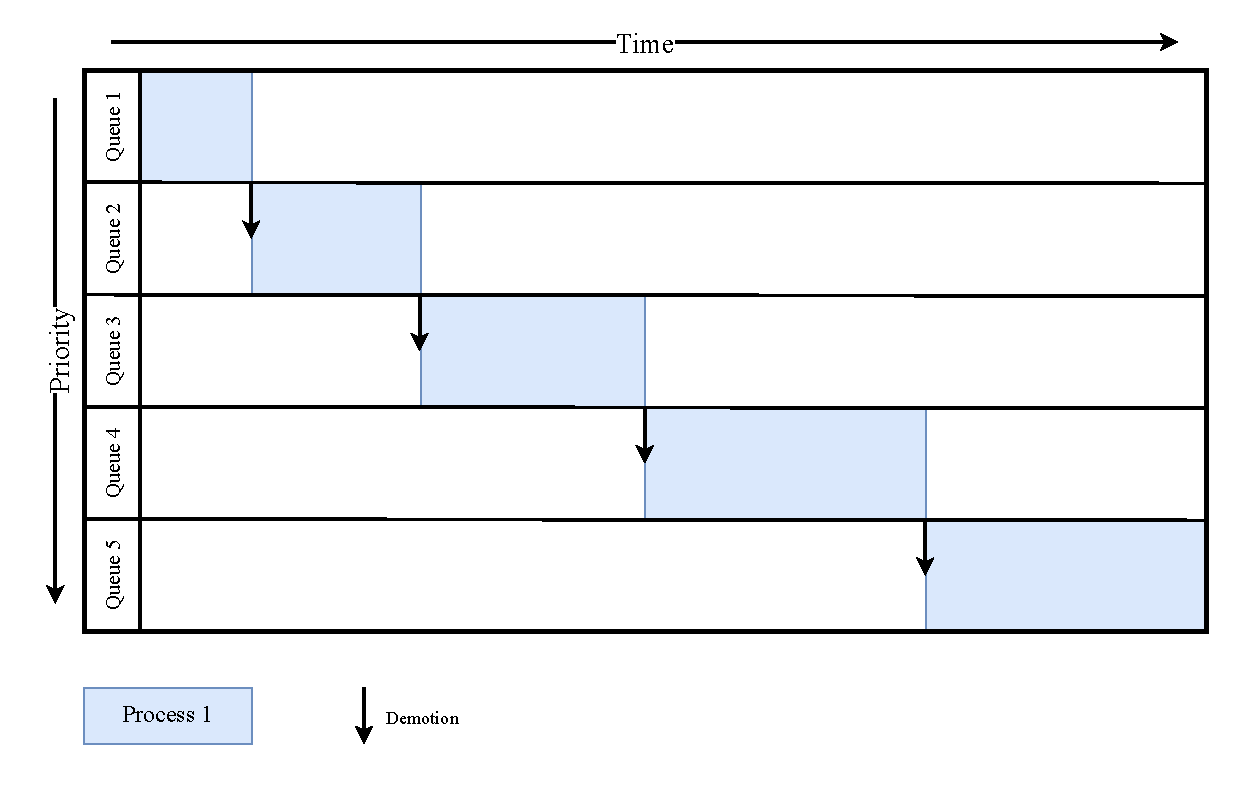
\includegraphics[width=0.7\textwidth]{Assets/MLFQ-Example-1.pdf}
    \caption{Simple working of MLFQ}
    \label{fig:mlfq-example-1}
\end{figure}


As you can see in figure \ref{fig:mlfq-example-1} the process one gets demoted after a while.
Also the lower the queue is, the higher the allotment time. 
This is because we hope that all of the responsive focused finish before demoting.
Once these are filtered out we have only resource heavy tasks left.
These require more time anyways, so the allotment time is stretched out.

\section{Multiple Processes}

What happens if we introduce another process?
Well, it depends on the priorities. 
Higher priority recieves the CPU time.
If they are on the same queue, than they run using Round Robin, see section \ref{sec:rr}.


\begin{figure}[h]
    \centering
    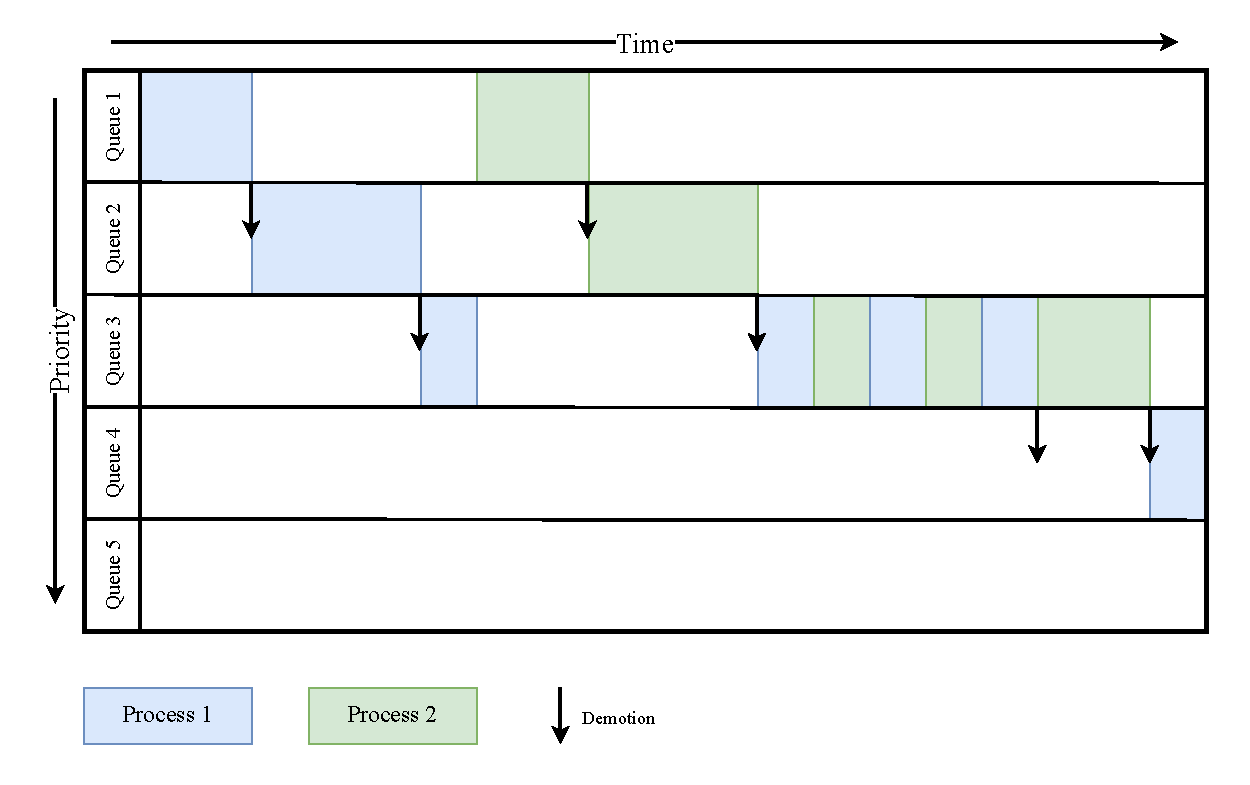
\includegraphics[width=0.7\textwidth]{Assets/MLFQ-Example-2.pdf}
    \caption{Running multiple processes in MLFQ}
    \label{fig:mlfq-example-2}
\end{figure}

As you can see in figure \ref{fig:mlfq-example-2} once process two is introduced process one is temporarily starved. The problem is solved once they land on the same queue.
There they run alternately.
Still the more tasks we introduce the more prevalent the starving issue gets.

\begin{figure}[h]
    \centering
    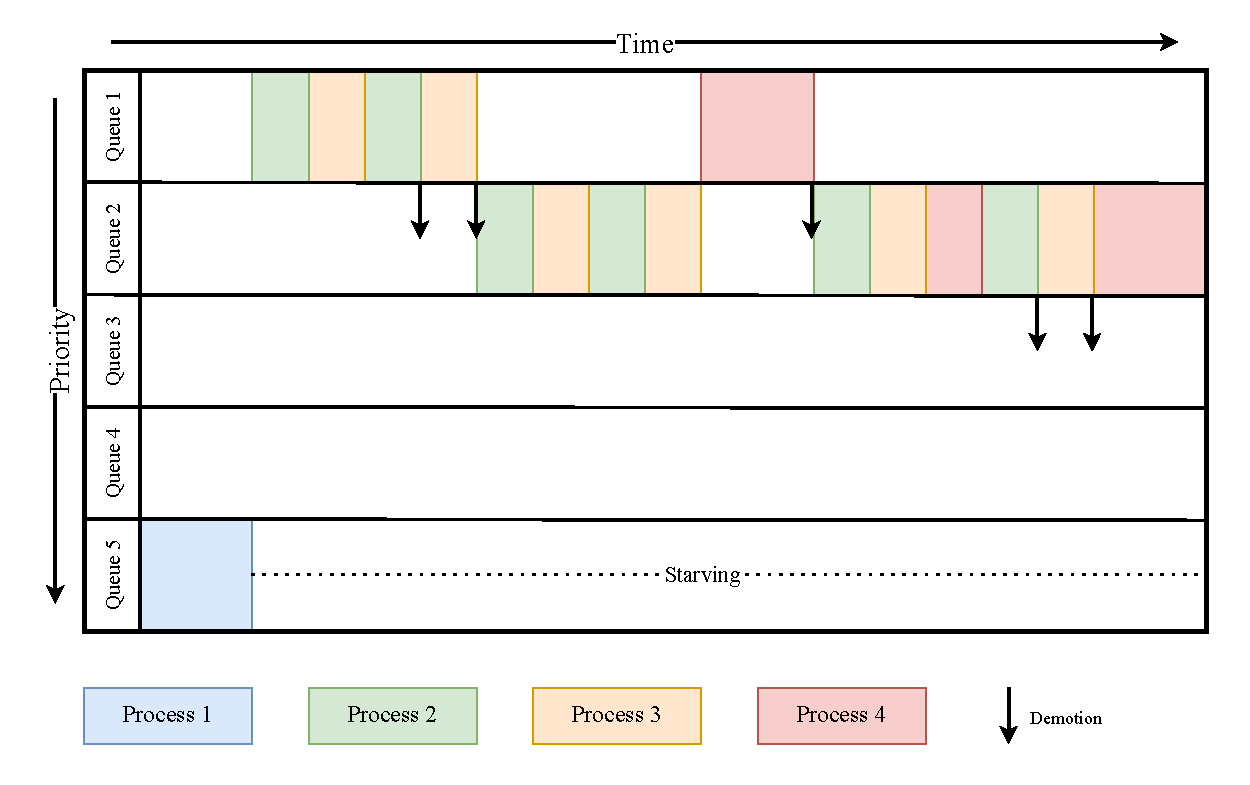
\includegraphics[width=0.7\textwidth]{Assets/MLFQ-Example-3.pdf}
    \caption{Starving Processes in MLFQ}
    \label{fig:mlfq-example-3}
\end{figure}



          % This ensures that the subsequent sections are being included as root
          % items in the bookmark structure of your PDF reader.
          \bookmarksetup{startatroot}
          \backmatter
          

          \begin{thebibliography}{99}
            \bibitem{ostep}
              Remzi Hussein Arpaci-Dusseau \& Andrea Carol Arpaci-Dusseau (2018) \emph{Operating Systems: Three Easy Pieces}, CreateSpace Independent Publishing Platform.
            \bibitem{coffman68}
              Edward G. Coffman \& Leonard Kleinrock (1968) \emph{Computer scheduling methods and their countermeasures}, Association for Computing Machinery.
            \bibitem{waldspurger95}
              Carl A. Waldspurger (1995) \emph{Lottery and Stride Scheduling: Flexible Proportional-Share Resource Management}, Massachusetts Institute of Technology.
            \bibitem{waldspurger94}
              Carl A. Waldspurger \& William E. Weihl (1994) \emph{Lottery scheduling: Flexible proportional-share resource management}, Massachusetts Institute of Technology.
            \bibitem{solaris}
              Andrea Carol Arpaci-Dusseau (2000) \emph{Multilevel Feedback Queue Scheduling in Solaris}, available at: \url{https://pages.cs.wisc.edu/~remzi/OSTEP/Citations/notes-solaris.pdf}
          \end{thebibliography}

          \section*{Further Sources}
          \begin{itemize}
            \item \url{https://github.com/Pseudomanifold/latex-mimosis}
            \item \url{https://en.wikipedia.org/wiki/Binary_search}
            \item \url{https://www.quora.com/Why-is-look-up-faster-for-a-Binary-Tree-than-a-Linked-List}
            \item \url{https://ceunican.github.io/aos/09.Scheduling_Proportional_Share.pdf}
            \item \url{https://courses.cs.washington.edu/courses/cse451/12au/l11.pdf}
            \item \url{https://en.wikipedia.org/wiki/Earliest_eligible_virtual_deadline_first_scheduling}
            \item \url{https://en.wikipedia.org/wiki/Proportional_share_scheduling}
            \item \url{https://www.youtube.com/watch?v=MkJfuI5_hjc&t=29s}
            \item \url{https://www.youtube.com/watch?v=qvZGUFHWChY&list=PL9xmBV_5YoZNqDI8qfOZgzbqahCUmUEin&index=1&pp=iAQB}
            \item \url{https://www.youtube.com/watch?v=95s3ndZRGbk&list=PL9xmBV_5YoZNqDI8qfOZgzbqahCUmUEin&index=2&pp=iAQB}
            \item \url{https://en.wikipedia.org/wiki/Red%E2%80%93black_tree} 
          \end{itemize}


          \end{document}
